\documentclass{article}
\usepackage{spconf,amsmath,graphicx}
\usepackage{amssymb}
\usepackage{enumitem}
\usepackage{hyperref}

\title{Optimizing DTW-Based Audio-to-MIDI Alignment and Matching}

\name{Colin Raffel and Daniel P. W. Ellis}
\address{LabROSA\\
    Columbia University\\
    New York, NY}

\begin{document}
\ninept
\maketitle

\begin{abstract}
Dynamic Time Warping (DTW) has proven to be an extremely effective method for both aligning and matching recordings of songs to corresponding MIDI transcriptions.
The performance of DTW-based approaches in this domain is heavily effected by system design choices, such as the representation used for the audio and MIDI data and DTW's adjustable parameters.
We propose a method for optimizing the design of DTW-based alignment and matching systems.
Our technique uses Bayesian optimization to tune system design and parameters over a synthetically created dataset of audio and MIDI pairs.
We then perform an exhaustive search over DTW score normalization techniques in order to determine an optimal method for reporting a reliable alignment confidence score, which is necessary for matching tasks.
Using our approach, we are able to create a DTW-based system which is conceptually simple and highly accurate at both alignment and matching.
We also verified that our system achieves high performance in a large-scale qualitative evaluation of results on real-world data.
\end{abstract}

\begin{keywords}
Dynamic Time Warping, Audio to MIDI Alignment, Sequence Retrieval, Bayesian Optimization, Hyperparameter Optimization
\end{keywords}

\section{Introduction}
\label{sec:intro}

MIDI files can provide a bounty of ground-truth data for content-based music information retrieval (MIR) tasks, including beat/bar tracking, onset detection, key estimation, automatic transcription, and score-informed source separation \cite{ewert2012towards, turetsky2003ground, ewert2014score, raffel2014pretty_midi}.
However, in order to utilize this data, a given MIDI file must first be aligned in time to a recording of the piece it is a transcription of.
A related problem is MIDI-to-audio matching, where we are given separate collections of MIDI and audio files and must determine which audio file (if any) each MIDI file corresponds to.
This problem is motivated by the dearth of metadata information typically available in MIDI files, making any kind of text-based matching infeasible \cite{raffel2015large}.
With or without useful metadata, it is beneficial to be able to produce a confidence score for alignment which communicates how well the content in a MIDI file matches a given audio file, which can help determine the transcription quality.

Despite these tasks' complementary nature, most previous research has focused on systems meant for either alignment or matching.
In the context of MIDI-to-audio alignment, a wide variety of techniques have been used, which typically involve determining a correspondence between discrete times in the audio and MIDI file.
While approaches inspired by edit distance metrics such as Smith-Waterman \cite{ewert2012towards} and Needleman-Wunsch \cite{grachten2013automatic} have been used, arguably the most common approach is Dynamic Time Warping (DTW) \cite{muller2007dynamic}.
First proposed for comparing speech utterances \cite{sakoe1978dynamic}, DTW uses dynamic programming to find a monotonic alignment such that the total distance between aligned feature vectors is minimized.
This property makes it well-suited for audio-to-MIDI alignment when we expect that the MIDI is an accurate continuous transcription (i.e.\ without out-of-sequence or incorrect sections).

A nice property of DTW is its appropriateness as a measure of the ``similarity'' between two sequences.
This is thanks to the fact that the total distance between pairs of feature vectors in the DTW-based alignment can be used reliability as a distance metric.
In fact, DTW has seen extensive use solely as a way of measuring sequence similarity in the data mining literature \cite{berndt1994using}.
In the context of MIDI and audio files, \cite{hu2003polyphonic} evaluated the effectiveness DTW distance to match a small collection of Beatles MIDIs to recordings of Beatles songs.

Despite its widespread use, DTW's success can be highly dependent on its exact formulation as well as system design choices such as the feature representation and the local distance metric used.
To our knowledge, there has been no large-scale quantitative comparison of different DTW-based alignment systems.
This is likely due to the fact that evaluating its performance would require either a collection of MIDI and audio pairs for which the correct alignment is already known (which does not exist) or manual audition and rating of the output of the system (which is time-consuming).
The present work aims to remedy this and produce a DTW-based alignment system which is optimal in terms of both alignment and matching accuracy.

After giving an overview of typical DTW-based alignment systems (Section \ref{sec:dtw}), we propose a method for creating a synthetic dataset of MIDI-audio pairs by applying realistic corruptions to MIDI files, which allows us to know a priori the correct alignment (Section \ref{sec:synthetic}).
We then tune parameters for alignment using Bayesian optimization (Section \ref{sec:optimizing}) and for confidence reporting using an exhaustive search (Section \ref{sec:confidence}).
Finally, we perform a large-scale qualitative evaluation of our proposed alignment system on real-world data and discuss possible avenues for improvement (Section \ref{sec:qualitative}).

\section{DTW-Based Alignment}
\label{sec:dtw}

Suppose we are given two sequences of feature vectors $X \in \mathbb{R}^{M \times D}$ and $Y \in \mathbb{R}^{N \times D}$, where $D$ is the feature dimensionality and $M$ and $N$ are the number of feature vectors in $X$ and $Y$ respectively.
Dynamic Time Warping produces two sequences $p, q \in \mathbb{N}^L$ which define the optimal alignment between $X$ and $Y$, such that $p[i] = n, q[i] = m$ implies that the $m$th feature vector in $X$ should be aligned to the $n$th in $Y$.
In DTW, finding $p$ and $q$ involves solving the following minimization problem:
$$
p, q = \mathrm{arg}\min_{p, q} \sum_{i = 1}^{L} \|X[p[i]] - Y[q[i]]\|_2^2 + \Phi(i)
$$
where $\Phi(i)$ is $\phi$ when $p[i] = p[i - 1]$ or $q[i] = q[i - 1]$ and $0$ otherwise.
$\phi \ge 0$ is a constant which is used to discourage ``non-diagonal moves'', i.e.\ indices in the path where one feature vector in one sequence is mapped to multiple vectors in the other.
This minimization problem can be solved in $\mathcal{O}(MN)$ time using dynamic programming \cite{sakoe1978dynamic}.
Once $p$ and $q$ are found, the original MIDI file can be adjusted so that events which occur at $t_X[p[i]]$ are moved to $t_Y[q[i]]$, where $t_X \in \mathbb{R}^M, t_Y \in \mathbb{R}^N$ are the times corresponding to the feature vectors in $X$ and $Y$ respectively.

Traditionally, DTW is constrained such that $p$ and $q$ span the entirety of $X$ and $Y$, i.e.\ $p[1] = q[1] = 1$ and $p[L] = N; q[L] = M$.
However, audio-to-MIDI alignment typically allows subsequence matching (a desireable case, for example, when a MIDI file is a transcription of a portion of a song), where instead we only require that either $gN \le p[L] \le N$ or $gM \le q[L] \le M$.
$g \in [0, 1]$ (the ``gully'') is a parameter which determines the proportion of the subsequence which must be successfully matched.
In addition, the path is occasionally further constrained so that
\begin{equation}
q[i] - p[i] + R \le N, p[i] - q[i] + R \le M
\end{equation}
for $i \in \{1, \ldots, L\}$ where $R = g\min(M, N)$ is the ``radius'', sometimes called the Sakoe-Chiba band \cite{sakoe1978dynamic}.
A further constraint on $p$ and $q$ is monotonicity, i.e.\ that
$$
p[i + 1] \ge p[i], q[i + 1] \ge q[i] \; \forall i
$$
This can be enforced by allowing a specific ``step pattern''; while many exist \cite{muller2007dynamic, sakoe1978dynamic}, to our knowledge the only pattern used in audio to MIDI alignment simply requires that
$$
(p[i + 1], q[i + 1]) \in \begin{cases}
(p[i] + 1, q[i] + 1)\\
(p[i], q[i] + 1)\\
(p[i] + 1, q[i])
\end{cases}
$$

From the above definition, it is clear that there are many design choices to be made when performing DTW-based audio-to-MIDI alignment:
\begin{description}[topsep=1pt,itemsep=-1pt,leftmargin=5pt]
\item[Feature representation ($X$ and $Y$):] Prior to alignment, audio and MIDI sequences must be converted to a common mid-level representation.
This is typically done by synthesizing the MIDI file to obtain an audio signal and computing a common spectral transform of the audio recording and synthesized MIDI audio.
Chroma vectors, which represent the amount of energy in each semitone summed across octaves \cite{fujishima1999realtime}, are a common choice \cite{hu2003polyphonic, ewert2012towards}.
A constant-Q transform (CQT), which represents the amount of energy in logarithmically spaced bins \cite{brown1991calculation} has also been used \cite{raffel2015large, dixon2005match, ellis2013aligning}.
Occasionally, log-magnitude features are used in order to more closely mimic human perception \cite{raffel2015large, ellis2013aligning, turetsky2003ground}.
In \cite{turetsky2003ground} and \cite{hu2003polyphonic} it is noted that Mel-Frequency Cepstral Coefficients result in poor performance for music signals because they discard pitch information.
\item[Time scale ($t_X$ and $t_Y$):] Feature vectors are frequently computed over short, overlapping frames of audio \cite{dixon2005match, turetsky2003ground, hu2003polyphonic}.
Note that the spacing between feature vectors must be sufficiently small compared to the auditory temporal resolution, e.g.\ tens of milliseconds \cite{blauert1997spatial}.
Occasionally, beat-synchronous feature vectors are used \cite{raffel2015large,ellis2013aligning}, which can dramatically reduce computation time and can produce perceptually accurate alignments provided that the beat tracking is correct.
\item[Normalization:] In \cite{rakthanmanon2012searching}, it is argued that z-scoring (standardizing) the feature sequences is critical for data mining applications of DTW, which was used in audio-to-MIDI alignment in \cite{hu2003polyphonic}.
In addition, various normalizations have been applied to the feature vectors in $X$ and $Y$ before computing their local distances.
A common choice is normalizing by each vector by its $L^2$ norm, which effectively results in the local distance being the cosine distance \cite{turetsky2003ground, ewert2012towards, raffel2015large, ellis2013aligning}.
\item[Penalty ($\phi$):] In many applications of DTW to audio-to-MIDI alignment, no additive penalty is used, which corresponds to setting $\phi = 0$.
However, as long as the MIDI and audio files have consistent tempi, non-diagonal moves should be discouraged.
In addition, it has been argued \cite{raffel2015large} that when the constraint $p[1] = 1, q[1] = 1$ is not enforced (which allows subsequence alignment), an additive penalty can be crucial to ensure that the entire subsequence is used, and so $\phi$ is set to the 90th percentile of the distances $\|X[n] - Y[m]\|_2^2$ for $m \in \{1, \ldots, M\}; n \in \{1, \ldots, N\}$.
In \cite{ellis2013aligning}, a fixed value of $\phi = .5$ is used.
\item[Gully ($g$) and band path constraint:] As with $\phi$, the ``gully'' and band path constraint are often omitted, which corresponds to setting $g = 1$.
A value of $g$ which is close to 1 will afford some tolerance to the possibility that the beginning or end of the MIDI transcription is incorrect (e.g.\ a fade-out or lead-in), so \cite{ellis2013aligning} sets $g = .7$ and \cite{raffel2015large} sets $g = .95$.
In data mining applications \cite{ratanamahatana2004everything} it is argued that the band radius path constraint both reduces computational complexity and results in more reliable alignments by avoiding paths with many non-diagonal moves.
\end{description}

\section{Creating a Synthetic Alignment Dataset}
\label{sec:synthetic}

From the discussion above, it is clear that there is a large space of parameter settings/design choices for DTW-based audio-to-MIDI alignment systems.
To our knowledge, previous researchers have mainly manually tuned alignment parameters based on a small test set of MIDI/audio pairs and have chosen the system which gives good qualitative results by audition of the aligned MIDI data.
Because this method only facilitates small-scale comparisons, there is an obvious question of what parameter settings would yield the best general-purpose alignment system.
Unfortunately, manual audition of even a tiny subset of possible parameter settings on a modestly-sized collection of paired MIDI and audio files is infeasible, let alone a collection large enough to make substantive judgements about the general performance of a given system.
Furthermore, automatic evaluation has not been an option due to the lack of a ground-truth dataset of ``correct'' alignments.
We therefore propose a method for synthetically creating a collection of MIDI/audio pairs by applying a series of corruptions to MIDI files which mimic real-world data.
When applying the corruptions, we keep track of the correct adjustments needed to restore the corrupted MIDIs back to the correct timebase, which facilitates automatic comparison and allows us to rapidly and automatically a huge number of possible systems.

To create this dataset, we first collected 1,000 MIDI files which were transcriptions of Western popular music songs.
We then applied the following series of transformations, based on our experience with common differences between MIDI transcriptions and audio recordings:
First, to simulate differences in tempo, we adjusted the timing in each MIDI file by a low-frequency length-$N$ random signal, generated as
$$
r[n] = \sum_{k = 0}^{N - 1} \mathcal{N}(0, \sigma_t) e^{j2\pi kn/N - n}, n \in \{1, \ldots, N\}
$$
i.e.\ the inverse Fourier transform of an exponentially decaying Gaussian-distributed random spectra with standard deviation $\sigma_r$.
Second, the first 10\% and last 10\% of the transcription were each cropped out with probability 50\%, which simulates the MIDI file being an incomplete transcription.
In addition, 1\% of the transcription was cut out at a random location with 10\% probability, which simulates a missing measure.
Third, because it is common for a MIDI transcription to be missing an instrument (for example, karaoke versions of songs are frequently distributed as MIDI files, which do not contain a vocal instrument), we removed each instrument track in each MIDI file with probability $p_r$, making sure to never remove all instruments.
Fourth, in all MIDI files, we randomly added 1 or -1 to the program number of each instrument.
This simulated the fact that when comparing a synthesized MIDI file to an audio recording, the timbre of a synthesized MIDI instrument is always somewhat different from its real-world counterpart.
Finally, for each note in each instrument, we multiplied the velocity by a random number sampled from $\mathcal{N}(1, \sigma_v)$ while keeping it in the MIDI velocity range $[1, 127]$.
This was meant to further simulate differences in instrument characteristics in real-world vs. synthesized songs, and also simulated missing notes for large $\sigma_v$.
All MIDI data manipulations were realized with \texttt{pretty\char`_midi} \cite{raffel2014pretty_midi}.

As described in Section \ref{sec:intro}, a DTW-based alignment system can serve two purposes: First, to align a MIDI transcription in time to an audio recording, and second, to produce a confidence score denoting the quality of the transcription or whether the MIDI file is a transcription of the recording at all.
We therefore produced two sets of corrupted version of the 1,000 MIDI files we collected, one each to measure the performance for alignment and confidence reporting.
For the first (``easy'') set, we focused on corruption parameters corresponding to real-world conditions for a high-quality transcription, setting $\sigma_t = 5, p_r = .1, \sigma_v = .2$.
For the second (``hard''), we set the corruption parameters so that the transcription was likely no longer valid, setting $\sigma_t = 20, p_r = .5, \sigma_v = 1$.

\section{Optimizing DTW-Based Alignment}
\label{sec:optimizing}

Given a dataset of MIDI/audio pairs where we know a priori the correct alignment, we can rapidly evaluate the performance of a given alignment scheme by aligning each pair and computing the mean absolute alignment error.
In the present setting, computing the mean error quantifies the extent to which the alignment was able to remove the timing distortions (random warping and cropping) described in Section \ref{sec:synthetic}.
When the alignment has failed for a portion of the song, the error between the mapped times and the correct times may be very large, so we clip the mean error to $.5$ seconds (which essentially denotes an error threshold above which all local alignment discrepancies are equally incorrect).
This results in the following metric for computing the accuracy of a given alignment scheme on a given MIDI/audio pair:
$$
\frac{1}{L}\sum_{i = 1}^{L} \min(|t_X[p[i]] - \hat{t}_X[q[i]]|, .5)
$$
where $\hat{t}_X$ is the ground-truth correct aligned timing.
To compute the accuracy of a given alignment system, we can compute the mean of this metric accross all pairs in the dataset.

The ability to rapidly evaluate an alignment system allows us to perform large-scale comparisons of different parameter settings.
To decide which parameter settings to evaluate, we use Bayesian optimization, which treats the process of tuning parameters to achieve different accuracies as a Gaussian process.
Using this formulation, Bayesian optimization can automatically propose new alignment systems based on the performance of previously evaluated systems.
As a performance objective, we used the mean of mean absolute errors across the entire ``easy'' alignment dataset.
A more thorough discussion can be found in \cite{snoek2012practical}, which is the framework we used in this experiment.

Before applying Bayesian optimization, we must define a parameter space to search over.
Based on the design choices outlined in Section \ref{sec:dtw}, we chose the following parameter space:
\begin{description}[topsep=1pt,itemsep=-1pt,leftmargin=5pt]
\item[Feature representation:] We used either chroma vectors or constant-Q spectra.
The constant-Q spectra spanned 4 octaves, starting from MIDI note C3 (65.4 Hz) with 12 bins per octave.
In preliminary experiments, we found that all of the best-performing alignment systems used log-magnitude features regardless of whether chroma vectors or constant-Q spectra were used, so we computed log-magnitude features in all experiments.
\item[Time scale:] We either computed feature vectors every 46 milliseconds or utilized beat-synchronous features.
\item[Normalization:] We optionally z-scored the feature vectors, and normalized feature vectors by their $L^1$, $L^2$, $L^\infty$ (max) norm, or not at all.
\item[Penalty:] For the penalty, we optimized a scale in $[0, 3]$ to apply to the median distance between all pairs of feature vectors in $X$ and $Y$.
Using the median distance made this penalty adaptive to different feature representations and normalization schemes.
\item[Gully and band path constraint:] We allowed the gully to take any value in $[0, 1]$ and optionally enforced the band path constraint (Sakoe-Chiba band).
\end{description}
This space subsumes most of the systems discussed in Section \ref{sec:dtw}.
All feature extraction was realized with \texttt{librosa} \cite{mcfee2015librosa}.

When performing Bayesian optimization, it is helpful to ``seed'' the optimization with objective values for many randomly-chosen parameter settings to ensure that the optimization thoroughly explores the possible parameter space.
We computed the accuracy for 10,000 randomly configured alignment systems and seeded the optimizer with the 100 systems which achieved the lowest mean error.
In order to avoid local minima in the parameter space, we carried out 10 separate Bayesian optimization runs with 100 trials each, resulting in 1,000 total trials.

The best-performing alignment system achieved an objective value of $0.0181$, meaning that the average absolute error across the entire dataset was about 18 milliseconds.
This is both within the upper range of the auditory temporal resolution and less than half of the time-scale resolution used for non-beat-synchronous feature vectors, so attaining a higher accuracy is likely unrealistic.
To find systems with comparably high performance, we performed a one-sample $t$-test to determine whether the difference between pairwise alignment errors from a given alignment system and those from the best system was significantly different than 0.
By using a test on the per-pair scores rather than the mean error across all pairs we achieve better robustness to outliers.
We considered an alignment system to not be significantly different from the best system if the $p$-value was greater than $.05$, which resulted in 51 alignment systems.

As a high-level overview of these systems, none used beat-synchronization or a path constraint and all of them used log-magnitude constant-Q spectra as a feature representation and set both the penalty median scale and ``gully'' close to 1.
Almost all of these systems used $L^2$ normalization (resulting in a cosine distance for local feature comparisons); a few used $L^1$ normalization.
Whether z-scoring was applied or not varied.

\section{Optimizing Confidence Reporting}
\label{sec:confidence}

Having found alignment systems which achieve high accuracy on the ``easy'' dataset, the question remains which of these systems can produce a reliable confidence score for a given alignment and how best to compute it.
As described in Section \ref{sec:dtw}, DTW provides a ``raw'' distance by simply summing the distances between all aligned feature vectors.
This metric is inappropriate, however, when the number of aligned feature vectors varies from song to song; in this setting, the mean distance is usually used instead of the total distance.
Furthermore, it is not immediately clear whether to include the non-diagonal path penalties $\phi$ in this distance.
Finally, in \cite{raffel2015large} it is advocated to further normalize this distance by
$$
\frac{1}{L^2} \sum_{i = \min(p)}^{\max(p)} \sum_{j = \min(q)}^{\max(q)} \|X[i] - Y[j]\|_2^2
$$
i.e.\ the mean distance between all pairs of frames over the entire aligned portion of both feature sequences.

To choose an optimal confidence score reporting method, we first aligned all of the MIDI/audio pairs in both the ``hard'' and ``easy'' datasets.
Then, for every alignment system generated during our Bayesian optimization trials, we computed the confidence score for every MIDI/audio pair using all combinations of the normalization schemes listed above (resulting in 8 possible confidence scores per file pair).
Finally, we computed the Kendall rank correlation coefficient \cite{kendall1938new} between each confidence score and the mean absolute error produced by all alignment systems for every alignment pair in both datasets.
A high correlation for a given confidence score for a given alignment system would indicate that the system is able to accurately report the quality of its alignments.

Among the 51 systems which were not significantly different from the highest-accuracy system on the ``easy'' dataset, the highest achieved correlation was 0.710.
In general, the high-accuracy systems all produced rank correlations which were close to this value.
All of the systems achieved the highest correlation when including the penalties in the score calculation, normalizing by the path length, and normalizing by the mean distance across the aligned portions.
This suggests that these steps are helpful for producing a reliable confidence score.

As a final step in producing a ``gold standard'' alignment system, we decided to find parameter settings which were easier to report and implement but nevertheless produced alignments and confidence scores which were not significantly different than the best systems.
We chose the following design: For a feature representation, we used log-magnitude constant-Q transforms computed on the non-beat-synchronous time scale described in Section \ref{sec:optimizing}.
We normalized the spectra by their $L^2$ norm and did not z-score them.
We chose a penalty $\phi$ as the median distance of all pairs of frames and used a gully parameter $g$ of $0.96$.
This system achieved an alignment accuracy on the ``easy'' dataset of 0.0188, with alignment errors which were not significantly different from the best-performing system.
By normalizing the DTW distance (including penalties) by the path length and the mean distance across aligned portions, we achieved a correlation of 0.700.
This ``gold standard'' system is straightforward to implement, and will be used for the remainder of this work.

\section{Qualitative Evaluation of Real-World Data}
\label{sec:qualitative}

In the experiments described above, we have found a system which can achieve both high accuracy and useful confidence reporting on synthetic data.
To determine its applicability outside of synthetic contexts, we performed a large-scale qualitative evaluation on real-world data.
The dataset used was a subset of 500 MIDI/audio pairs from the ``clean MIDI dataset'' \cite{raffel2015large}, obtained by matching MIDI files with reliable metadata to entries in the Million Song Dataset via a fuzzy text match.
This collection comprises MIDI files with a full range of transcription qualities, and includes some pairs which are incorrectly matched due to failure of the text matching procedure.
By manually evaluating whether each resulting alignment was successful, we can determine how accurately it performs alignments and how reliable the reported confidence scores are.

After aligning all pairs in this dataset using the ``gold standard'' system, we synthesized the resulting aligned MIDI files and created stereo recordings which consisted of the aligned synthesized MIDI audio in one channel and the original audio recording in the other.
We then listened to each aligned MIDI pair and annotated a score from 1-5 according to the alignment accuracy, as follows:
\begin{enumerate}[topsep=1pt,itemsep=-1pt]
\item MIDI and audio file are incorrectly matched
\item Alignment failed due to major differences
\item Alignment was mostly successful with minor issues
\item Perfect alignment with minor transcription issues
\item Perfect alignment and transcription
\end{enumerate}
For example, if a MIDI transcription was matched and successfully aligned to the correct song but was missing a transcription of the song's vocals, a rating of 4 would be given; if the missing vocals caused the alignment to sound ``sloppy'', the rating would be 3 instead.

\begin{figure}[t]
  \label{fig:violin}
  \centering
  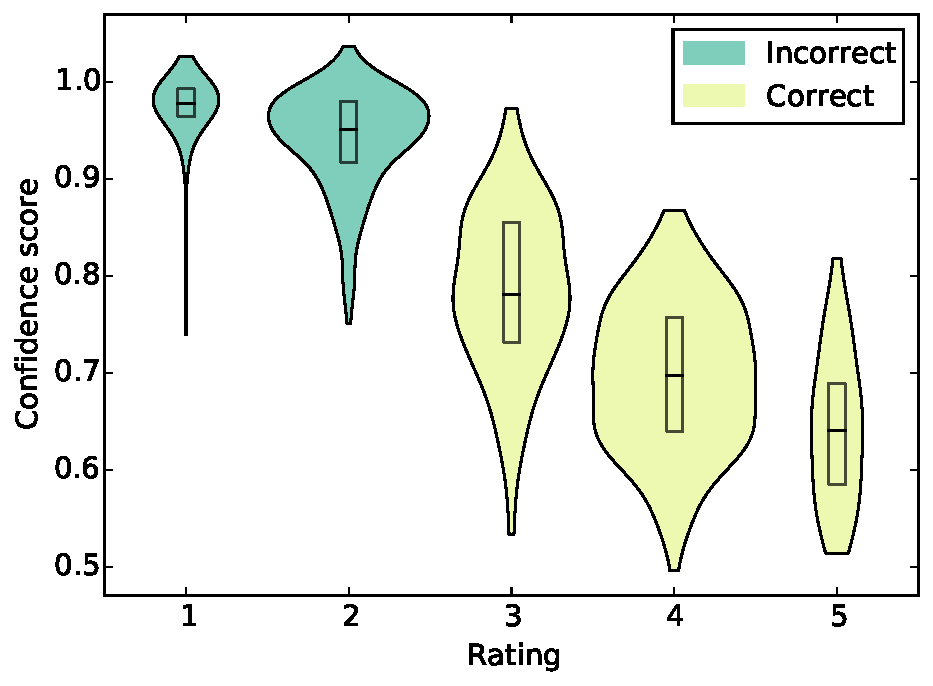
\includegraphics[width=\columnwidth]{violin.pdf}
  \caption{Violin plot showing the distribution of confidence scores for each rating in our qualitative evaluation.
A smaller confidence score indicates a more successful alignment.
The area of each violin corresponds to the number of pairs which had a given rating.
Box plots in each violin show the median and upper and lower quartiles.}
\end{figure}

Figure \ref{fig:violin} shows the distributions of confidence scores for pairs assigned each of the five ratings.
In an ideal world, all MIDI and audio files would be paired correctly, and all MIDI transcriptions would be perfect.
However, apart from encountering many incorrect pairs (all of those rated 1), we also found that various transcription issues prevented successful alignments.
The most common issue resulting in a score of 2 was that the wrong section of the MIDI transcription was chosen to match the audio file, which was often due to very different instrumentation, different keys, or different versions (e.g.\ the audio recording was a live version).
Many pairs rated 3 had multiple missing instruments, many musical embellishments, or in some rare cases, were transcribed at the wrong tempo.
In addition, the large overlap between the confidence scores for pairs rated 4 and 5 indicates that our confidence score is largely invariant to minor transcription issues, which is not ideal.
The most common transcription issue for pairs rated 4 was a single missing instrument or minor embellishments, both of which most frequently effected the vocal track.

Despite these issues, our ``gold standard'' alignment system was able to successfully align most correctly matched pairs and produced an extremely reliable confidence score.
In fact, if we consider ``correct'' matches to be those rated 3, 4, or 5, the resulting confidence scores afford an area under the ROC curve of 0.983 (95\% confidence interval [.973, .991], calculated by 1000-sample bootstrap), indicating a highly reliable metric.
Unfortunately, there were a few pairs which were rated 1 or 2 but nevertheless had a small normalized DTW score (indicating a successful alignment) visible as outliers in Figure \ref{fig:violin}; without these outliers, we could more confidently use a higher threshold below which alignments could safely be considered correct.
Besides this, the main avenue for improving the system would be to determine a way to make the confidence score more sensitive to missing instruments and musical embellishments.
Nevertheless, through our large-scale optimization over synthetic data, we have designed a DTW-based system which is simple to implement and achieves accurate and reliable results for both alignment and matching.
A high-level discussion of these results, with more figures and an implementation example of our ``gold standard'' system, is available online\footnote{abc}, as is all of the code used in these experiments \footnote{xyz}.

\bibliographystyle{IEEEbib}
\bibliography{refs}

\end{document}
